% SCHMT

%%%% TO LATE CROP THE PDF AT THE CORRECT SIZE FOR PLOTING: %%%%
% pdfcrop --margins '-0 -0 -80 -417' bn_simple.pdf ../bn_simple_crop.pdf

\documentclass{article}
\usepackage{dcolumn}
\usepackage{booktabs}
\usepackage{tikz}
\usetikzlibrary{positioning,shapes,arrows}

\newcolumntype{M}[1]{D{.}{.}{1.#1}}

\begin{document}

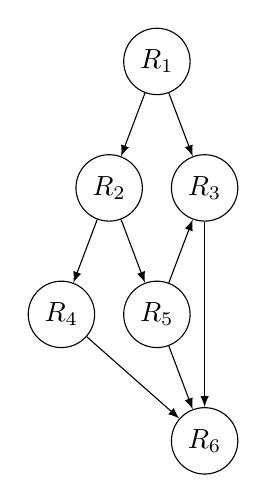
\begin{tikzpicture}[node distance=1cm and 0cm,
										mynode/.style={draw,circle,minimum width=0.5cm,align=center}
										]
	\node[mynode] (R1) {$R_{1}$};
	\node[mynode,below left=of R1] (R2) {$R_{2}$};
	\node[mynode,below right=of R1] (R3) {$R_{3}$};
	\node[mynode,below left=of R2] (R4) {$R_{4}$};
	\node[mynode,below right=of R2] (R5) {$R_{5}$};
	\node[mynode,below right=of R5] (R6) {$R_{6}$};
	\path (R1) edge[-latex] (R2) 
	(R1) edge[-latex] (R3) 
	(R2) edge[-latex] (R4) 
	(R2) edge[-latex] (R5) 
	(R5) edge[-latex] (R3)
	
	(R3) edge[-latex] (R6) 
	(R4) edge[-latex] (R6) 
	(R5) edge[-latex] (R6);

% 	\node[left=of R1,left=0.5cm of R1]
% 	{
% 	\begin{tabular}{cM{2}M{2}}
% 	\toprule
% 	& \multicolumn{2}{c}{Sprinkler} \\
% 	Rain & \multicolumn{1}{c}{T} & \multicolumn{1}{c}{F} \\
% 	\cmidrule(r){1-1}\cmidrule(l){2-3}
% 	F & 0.4 & 0.6 \\
% 	T & 0.01 & 0.99 \\
% 	\bottomrule
% 	\end{tabular}
% 	};
% 	\node[left=of R1,right=0.5cm of ra]
% 	{
% 	\begin{tabular}{M{1}M{1}}
% 	\toprule
% 	\multicolumn{2}{c}{Sprinkler} \\
% 	\multicolumn{1}{c}{T} & \multicolumn{1}{c}{F} \\
% 	\cmidrule{1-2}
% 	0.2 & 0.8 \\
% 	\bottomrule
% 	\end{tabular}
% 	};
% 	\node[left=of R1,below=0.5cm of gw]
% 	{
% 	\begin{tabular}{ccM{2}M{2}}
% 	\toprule
% 	& & \multicolumn{2}{c}{Grass wet} \\
% 	\multicolumn{2}{l}{Sprinkler rain} & \multicolumn{1}{c}{T} & \multicolumn{1}{c}{F} \\
% 	\cmidrule(r){1-2}\cmidrule(l){3-4}
% 	F & F & 0.4 & 0.6 \\
% 	F & T & 0.01 & 0.99 \\
% 	T & F & 0.01 & 0.99 \\
% 	T & T & 0.01 & 0.99 \\
% 	\bottomrule
% 	\end{tabular}
% 	};

\end{tikzpicture}

\end{document}